\section{Binary Code Matching Features}\label{sec:category}

In this section, we elaborate the features that we adopt to measure the similarity of two binary code segments.  As listed in Table \ref{tab:features}, these features fall into three categories. For each feature in Table \ref{tab:features}, the example and description are given in the following subsections. Features of structures and high-level semantics are extracted via static analysis, which is the functionality of step 2. Features of low-level semantics are extracted by emulation (step 6).


\subsection{Structural Features}\label{sec:category:structralFea}

3D-CFG~\cite{3d-cfg} depicts the CFG structure of a function at a high-abstraction level. It is used to measure the similarity between methods in/among bytecode of Android apps. The basic idea in \cite{3d-cfg} is to assign a structural 3D-coordinate value for each node in the control flow graph (CFG) of a method, then calculate the mass centroid of these coordinates as the centroid of the method. By calculating the distance between two methods' centroids, the similarity among these two methods can be measured.

According to \cite{3d-cfg}, for a given method, each node in the CFG is a basic code block. Each node has a unique coordinate, denoted as a 3-tuple $(x, y, z)$, where $x$ is its sequential number in the CFG; $y$ is the number of its outgoing edges (out-degree of the node in CFG), and $z$ is the loop depth of the node.

Based on the nodes inside the function $f$, we define the  centroid $\overrightarrow{c_f}$ of  function $f$:


\begin{mydef}\label{thm:cdd} The centroid is a 4-tuple $(c_{x}, c_{y}, c_{z}, w)$~\cite{3d-cfg}:
\begin{itemize}[itemsep=0.1mm]
  \item $w~=~\sum_{e(p,q)\in3D-CFG}(w_{p}+w_{q})$,
    \item $c_{i}~=~\frac{\sum_{e(p,q)\in3D-CFG} (w_{p}i_{p}+w_{q}i_{q})}{w}, where~i\in\{x,y,z\}$
\end{itemize}\vspace{-1mm}
\end{mydef}
\noindent where $e(p,q)$ is the edge between the node $p$ and $q$, $(x_{p}, y_{p}, z_{p})$ is the coordinate of the node $p$, and $w_{p}$ is the number of assembly instructions in the node of BB.

To emphasize the importance of function call instruction (relevant to high-level semantics), the weighted centroid is defined as $\overrightarrow{c_f}' = ({c}_{x}', {c}_{y}', {c}_{z}', w')$ for function $f$, where $w' = w + N$, and $N$ is the number of function call instructions; ${c}_{x}',~{c}_{y}'$ and ${c}_{z}'$ are recalculated according to the new weight $w'$, respectively. Suppose each BB node in Fig.~\ref{fig:strucFea} contains only one instruction ($w_A=1, w_B=1, w_D=1$), and node $C$ contains one function call instruction  ($w_C=2$). We have the following coordinates: $(1,2,1)$ for $A$, $(2,2,1)$ for $B$, $(3,1,0)$ for $C$ and $(4,0,0)$ for $D$. Then, the centroid is \xyx{$(2.2,1.5,0.6,10)$} and the weighted centroid is \xyx{$(2.38,1.38,0.46,13)$}. %(where $w=10$, $N=1$ and $w'=13$).
%For example, for the first method in Fig.~\ref{fig:motivation}(a), the centroid is $(1,0,0,5)$ and the weighted centroid is $(1,0,0,9)$ (only four invocation statements). Note that $w'$ is 9, the sum of $w$  and the number of invocation statements.

Given a function $f$, the function signature $\overrightarrow{f} =(\overrightarrow{c_f}, \overrightarrow{c_f}')$ is a feature vector containing the structural  information of the function, where  $\overrightarrow{c_f}$ is the centroid, $\overrightarrow{c_f}'$ is the weighted centroid.

The difference between the centroids of two functions $f_1$ and $f_2$ is the primary condition to evaluate their similarity:
 
\begin{mydef}\label{thm:cdd}
The Centroid Difference Degree (CDD)~\cite{3d-cfg} of two centroids $\overrightarrow{c_1} =({c_1}_{x}, {c_1}_{y}, {c_1}_{z}, w_1)$, $\overrightarrow{c_2}=({c_2}_{x}, {c_2}_{y}, {c_2}_{z}, w_2)$
(the distance of the weighted centroids  $\overrightarrow{c_1}'$ and $\overrightarrow{c_2}'$) is
 
\begin{small}
\begin{center}
$
CDD(\overrightarrow{c_1}, \overrightarrow{c_2}) = max(\frac{|{c_1}_x-{c_2}_x|}{{c_1}_x+{c_2}_x}, \frac{|{c_1}_y-{c_2}_y|}{{c_1}_y+{c_2}_y},\frac{|{c_1}_z-{c_2}_z|}{{c_1}_z+{c_2}_z},\frac{|w_1-w_2|}{w_1+w_2}) \nonumber
$
\end{center}
\end{small}
\end{mydef}

Given two functions, the function-level difference degree is defined as the maximum value between their centroid distance (CDD) and their weight centroid distance (weighted CDD):

\begin{mydef}
Function Difference Degree (FDD) of two functions $\overrightarrow{f_{1}}=(\overrightarrow{c_{1}}, \overrightarrow{c_{1}}' )$ and $\overrightarrow{f_{2}}=(\overrightarrow{c_{2}}, \overrightarrow{c_{2}}' )$ is
{
\begin{small}
\begin{center}

$FDD(\overrightarrow{f_{1}}, \overrightarrow{f_{2}}) = max(CDD(\overrightarrow{c_{1}}, \overrightarrow{c_{2}}),CDD(\overrightarrow{c_{1}}', \overrightarrow{c_{2}}'))$
\end{center}
\end{small}
}
\end{mydef}

\begin{figure}[tb]
\begin{minipage}{0.5\linewidth}
\centering
\scriptsize
 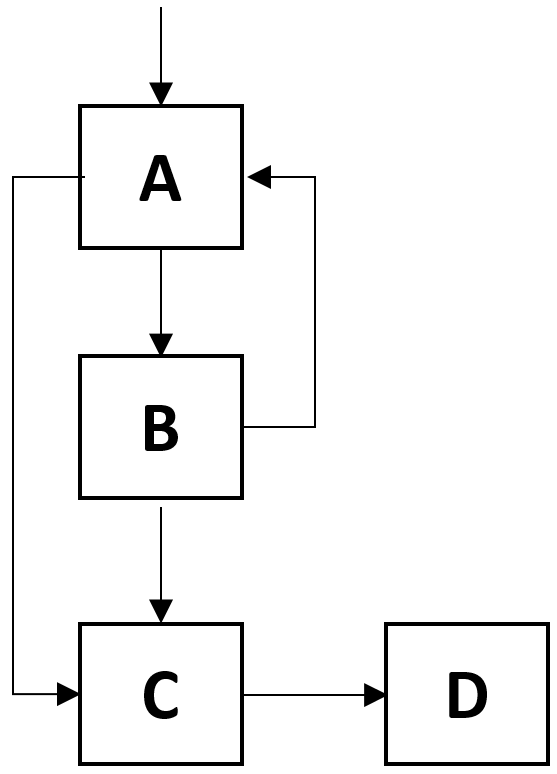
\includegraphics[width=2 cm]{srj-figures/3d-cfg.png}
%\\[0.2cm] (a) candidate DFA $\mathcal{C}_1$
\end{minipage}
~
\begin{minipage}{0.5\linewidth}
\centering
\scriptsize
\begin{tabular}{l} \hline
\textbf{Structural features:} \\
BB sequence: \\
~~~~main: $A \to B \to C \to D$ \\
~~~~the sequential number of BB (A): $1$ \\
In-degree of BB (A): $2$ \\
out-degree of BB (A): $2$ \\
Loop information: \\
~~~~The loop depth of BB (A): $1$ \\
~~~~involving number of BBs: $2$ \\
\hline
\end{tabular}
%\\[0.2cm] (b) candidate DFA $\mathcal{C}_2$
\end{minipage}
\vspace{-2mm}
\caption{The BB-structure of a function, and its structural features
}
\label{fig:strucFea}
\end{figure}

The two code segments in Fig.~\ref{fig:falseposi} will not be matched as similar according to these structural features. \xyx{Since the code segment in Fig.~\ref{fig:falseposi:a} has only one BB and the code segment in Fig.~\ref{fig:falseposi:b} has 3 BBs. Their CDD and weighted CDD are all 1 ($c_{1y}$ and $c_{1z}$ are all 0), which indicates zero similarity  according to~\cite{3d-cfg}\cite{DBLP:conf/issta/MengXXLZN16}.  Thus, 3D-CFG captures the overall structure of a binary function; and it is effective in measuring the structural similarity of two given binary functions.}

 \subsection{High-level Semantic Features}\label{sec:category:highSemanticFea}
For the high-level semantics, we mainly make use of the operation types, system call tags (tags of function calls to system APIs), function call sequences, function call parameters, local variables and op. code.  The basic idea is that  function calls (especially system calls) carry the semantics of code and they can be used for semantic-based code matching tasks,  e.g., system-call based malware detection~\cite{DBLP:conf/issta/CanaliLBKCK12}. Hence, the information of function calls (tags, parameters, sequences) is extracted as features. Additionally, we extract features from the numbers of different types of binary instructions. \xyx{We first classify different binary instructions into 15 categories\footnote{The instructions inside each category can be found from this link: \url{https://sites.google.com/site/toolbingoe/instruction-category}}, including \emph{data\_transfer}, \emph{arithmetic}, \emph{stack}, \emph{logical}, \emph{shift\_rotate}, \emph{control\_transfer}, \emph{loop}, \emph{string}, \emph{flag}, \emph{misc}, \emph{sign}, \emph{fstp}, \emph{port}, \emph{mmx}, \emph{call}.
Then we use the number of instructions in each category as a feature.} Last, we also extract features from local variables. The reason is that  local variables may represent the intermediate values in the execution, and the same intermediate values indicate the same or similar function semantics.




\begin{figure}[tb]
\begin{minipage}{0.5\linewidth}
\centering
\scriptsize
 \begin{tabular}{|l|}  \hline
$\mathtt{push \quad    ebp}$\\
$\mathtt{mov  \quad ebp, esp}$\\
$\mathtt{sub  \quad esp, 56}$\\
$\mathtt{sub  \quad esp, 8}$\\
$\mathtt{lea  \quad  eax, [ebp-16]}$\\
$\mathtt{push \quad   eax}$\\
$\mathtt{push \quad   OFFSET~FLAT:.LC0}$\\
$\mathtt{call \quad   scanf}$\\
$\mathtt{add  \quad    esp, 16}$\\
$\mathtt{mov  \quad    eax, DWORD~PTR [ebp-16]}$\\
$\mathtt{sub  \quad    esp, 12}$\\
$\mathtt{push \quad   eax}$\\
$\mathtt{call \quad   strlen}$\\
$\mathtt{add  \quad    esp, 16}$\\
$\mathtt{mov  \quad    DWORD~PTR [ebp-12], eax}$\\
$\mathtt{cmp  \quad    DWORD~PTR [ebp-12], 9}$\\
$\mathtt{jg   \quad    .L2}$\\
 \hline
\end{tabular}
\\[0.2cm] (a) basic block $B_1$\\
 \vspace{2mm}
 \begin{tabular}{|l|}
  \hline
$\mathtt{ mov \quad  eax, 0 }$~~~~~~~~~~~~~~~~~~~~~~~~~~~~~~~~\\
$\mathtt{leave}$\\
$\mathtt{ret}$\\
\hline
\end{tabular}
\\[0.2cm] (b) basic block $B_2$
\end{minipage}
~
\begin{minipage}{0.5\linewidth}
\centering
\scriptsize
 \begin{tabular}{|l|}  \hline
$\mathtt{mov \quad edx, DWORD~PTR [ebp-12]}$\\
$\mathtt{mov \quad    eax, DWORD~PTR [ebp-16]}$\\
$\mathtt{sub \quad    esp, 4}$\\
$\mathtt{push\quad    edx}$\\
$\mathtt{push\quad    eax}$\\
$\mathtt{lea \quad    eax, [ebp-56]}$\\
$\mathtt{push\quad   eax}$\\
$\mathtt{call\quad    memcpy}$\\
$\mathtt{add \quad    esp, 16}$\\
$\mathtt{mov \quad    eax, 10}$\\
$\mathtt{sub \quad    eax, DWORD~PTR [ebp-12]}$\\
$\mathtt{mov \quad    ecx, eax}$\\
$\mathtt{mov \quad    eax, DWORD~PTR [ebp-12]}$\\
$\mathtt{lea \quad    edx, [0+eax*4]}$\\
$\mathtt{lea \quad    eax, [ebp-56]}$\\
$\mathtt{add \quad    eax, edx}$\\
$\mathtt{sub \quad    esp, 4}$\\
$\mathtt{push\quad    ecx}$\\
$\mathtt{push\quad    32}$\\
$\mathtt{push\quad    eax}$\\
$\mathtt{call\quad    memset}$\\
$\mathtt{add \quad    esp, 16}$\\
 \hline
\end{tabular}
\\[0.2cm] (c) basic block $B_3$
\end{minipage}
\begin{minipage}{0.5\linewidth}
\centering
\scriptsize
\begin{tabular}{l}
%\textbf{High-level semantic features:} \\
~~\\\hline
 Op. type: \\
 $\quad data\_transfer(13),stack(10),$ \\
 $\quad  arithmetic(11), call(4), logical(1), $\\
 $\quad control\_transfer(1),  misc(1), $ \\
 System call tags: \\
  $\quad io, string, mem, mem $ \\
 Function call sequence:\\
  $\quad scanf \to strlen \to $\\
  $\quad memcpy \to memset$ \\
 Function parameter: Null\\
  %$\quad esp-24 (sub  esp, 24)$\\
 Local variable: \\
 $\quad  ebp-12 (mov [ebp-12], eax)$\\
  Op. code:\\
  $\quad   push \to mov \to  ... $\\
  $\quad    ... \to leave \to ret$\\
\hline
\end{tabular}
\\[0.2cm] (d) High-level semantic features of $B_1$, $B_2$ and $B_3$
\end{minipage}
~
\begin{minipage}{0.5\linewidth}
\centering
\scriptsize
\begin{tabular}{l}
$\mathtt{int~foo2()}$\\
\{\\
~~$\mathtt{char~\ast buf;}$\\
~~$\mathtt{char~\ast p[10];}$\\
~~$\mathtt{scanf(}$``\%s" $\mathtt{, \&buf);}$\\
~~$\mathtt{int~len;}$\\
~~$\mathtt{len = strlen (buf);}$\\
~~$\mathtt{if (len < 10)}$\{\\
~~~~      $\mathtt{memcpy (p, buf, len);}$\\
~~~~      $\mathtt{memset (p + len,}$`~'$\mathtt{, 10 - len);}$\\
~~\}\\
~~  $\mathtt{return 0;}$\\
\}\\

\end{tabular}
\\[0.2cm] (e)  the source code of these binary code segments
\end{minipage}
\caption{the high-level semantic features of an exemplar function}
\label{fig:highlevelFea}
\end{figure}

In Fig.~\ref{fig:highlevelFea}, we give an example for the high-level semantic features. \xyx{In  Fig.~\ref{fig:highlevelFea}(e), the semantics of the function $foo2$ is to do the string copy. Its binary code contains three BBs, in which $B_1$ has two out-edges to $B_2$ and $B_3$, and $B_3$ has one out-edge to $B_2$. The high-level semantic features in  Fig.~\ref{fig:highlevelFea}(d) are extracted from all the BBs of the function. Among all the instructions, we have 13 instructions of  \emph{data\_transfer}, 10 of \emph{stack},  4 of \emph{call}, 1 of \emph{control\_transfer}, and so on. Similar to the idea of mapping concrete system calls into abstract actions in~\cite{DBLP:conf/issta/CanaliLBKCK12}, we add tags to the common system calls or library calls in order to capture the high-level semantics of the function. For example, the tag of function call \emph{scanf} is \emph{io}, the tag of function call \emph{strlen} is \emph{string}, and the tag of \emph{memcpy} and  \emph{memset} is \emph{mem}\footnote{A more complete mapping list for function call tagging can be found from this link: \url{https://sites.google.com/site/toolbingoe/system-call-tags}}. Similar to the idea of using API usage patterns for code recommendation~\cite{DBLP:conf/ecoop/ZhongXZPM09} (source code search), we also extract the function call sequences on the longest program path: \small{$scanf \to strlen \to memcpy \to memset$} on the control flow $BB_1 \to BB_3 \to BB_2 $}. Function $foo2$ takes no parameters, and has the value of $null$ for this feature. Local variables used in source code  is  \small{$len$}, which stores the return value of function call \small{$strlen$} in Fig.~\ref{fig:highlevelFea}(e). Hoverer, in the binary code ($B_1$ in Fig.~\ref{fig:highlevelFea}(a)), the address at \small{$ebp-12$} stores the return value of function call \small{$strlen$} (according to the instruction ``$\mathtt{push~eax}$" that stores the return value of ``$\mathtt{call~strlen}$" into $\mathtt{eax}$  and the instruction ``$\mathtt{mov~DWORD~PTR [ebp-12], eax}$"). So we use the memory address \small{$ebp-12$}  as the feature for local variable. Last, the instruction types for all instructions in all BBs are used as a feature.

The two code segments of the false positive case in Fig.~\ref{fig:falseposi} is not matched as similar according to these high-level features. \xyx{Code segment in Fig.~\ref{fig:falseposi:a} has function call, while code segment in Fig.~\ref{fig:falseposi:b} does not. They also have different local variables  and opcode. For example, local variables are $\mathtt{ebp-12}$ and $\mathtt{ebp-16}$ in Fig.~\ref{fig:falseposi:a}, while they are $\mathtt{ebp-4}$ and $\mathtt{ebp-8}$ in Fig.~\ref{fig:falseposi:b}. Therefore, high-level semantic features are very helpful in recovering function semantics.}


\subsection{Low-level Semantic Features}\label{sec:category:lowSeFea}
\xyx{The basic idea of capturing low-level semantic features is to compare the input/output pair \cite{luo2014semantics}\cite{DBLP:conf/sp/PewnyGGRH15}, or compare the frequencies of different types of memory operations~\cite{egele2014blanket}. In \textsc{\tool}, features of input/output pairs are adopted for comparison (\S~\ref{sec:category:lowSeFea:io}). In \toolNew, as emulation is supported to improve the efficiency, we extend the approach to support features that are based on values (including intermediate values) read from (or written to) the program stack and heap (\S~\ref{sec:category:lowSeFea:freq}}).

\subsubsection{Features Used in \textsc{\tool}}\label{sec:category:lowSeFea:io}
  Similar to~\cite{luo2014semantics} and~\cite{DBLP:conf/sp/PewnyGGRH15}, a set of symbolic formulas (called \textit{symbolic expressions})
%(called, Input/Output or I/O formula)
are extracted from each partial trace, where they capture the effects of executing the partial trace on the machine state. Here, machine state is characterized by a 3-tuple $\langle mem, reg, flag\rangle$ denoting the memory \emph{mem}, general-purpose registers \emph{reg} and the condition-code flags \emph{flag}~\cite{DBLP:conf/sp/PewnyGGRH15, luo2014semantics}. For example, a machine state, before executing a partial trace, is given by $\mathcal{X} = \langle mem, reg, flag\rangle$, then just immediately after execution, the machine state is given by $\mathcal{X}^\prime = \langle mem^\prime, reg^\prime, flag^\prime \rangle$. Here, $\mathcal{X}$ and $\mathcal{X}^\prime$ are referred to as \textit{pre-} and \textit{post-state}, respectively, and the symbolic expressions capture the relationship between these pre- and post-machine states.

%a set of I/O formulas is extracted from each partial trace, and these formulas capture the relationship between symbolic pre- and post-state values. However, the extracted I/O formulas cannot be directly fed into our machine learning module. Hence, we leverage on the constraint solver to extract features by solving the formulas, where solving refers to finding appropriate values for the input and output vocabularies
In order to measure the similarity between the signature function and a target function, one can use a constraint solver, such as Z3~\cite{de2008z3}, to calculate the semantic \emph{equivalence} between the symbolic expressions extracted from the signature and target functions. However, using a constraint solver to measure semantic equivalence is very costly~\cite{luo2014semantics} and not scalable for real-world cases, considering the complexity of pair-wise matching between the signature function and a possibly huge number of target functions. To tackle the scalability issue, in~\cite{DBLP:conf/sp/PewnyGGRH15}, a machine learning technique is applied. Specifically, Input/Output (or I/O) samples are randomly generated from the symbolic expressions and are fed into the machine learning module to find semantically similar functions. Here, I/O samples are the input and output pairs --- assigning concrete values to the pre-state variables in the symbolic expressions and obtaining the output values of the post-state variables. %All these pairs of concrete input and output values constitute the I/O samples.

One of the drawbacks in randomly generating I/O samples is that the dependency among the symbolic expressions is ignored~\cite{DBLP:conf/sp/PewnyGGRH15}. For example, consider the following 2 symbolic expressions:%extracted from a single partial trace:\

\begin{eqnarray}
\scriptsize
\mathtt{zf^\prime \equiv (edx < 2) \wedge (edx > 0)} \label{eq:IO_1} \\
 \mathtt{ecx^\prime \equiv edx + 4} \label{eq:IO_2}
\end{eqnarray}
where symbolic expression 1 (Eq.~\ref{eq:IO_1}) has one pre-state (i.e., $\mathtt{edx}$) and one post-state variable (i.e., $\mathtt{zf}^\prime$), similarly, the symbolic expression 2 (Eq.~\ref{eq:IO_2}) also has one pre- (i.e., $\mathtt{edx}$) and one post- (i.e., $\mathtt{ecx}^\prime$) state variable. Thus these two symbolic expressions are mutually dependent through a common pre-state variable $\mathtt{edx}$. However, in randomly generated I/O samples (as in~\cite{DBLP:conf/sp/PewnyGGRH15}), $\mathtt{edx}$ can be assigned to two different values in each symbolic expression, which ignores the dependency and may lead to inaccurate semantics.

%It is necessary to ensure that the concrete value obtained for pre-state variable satisfies the both symbolic expressions.
%That is, for  $\mathtt{zf^\prime}$ to be $\mathtt{true}$, $\mathtt{edx}$ can only take the concrete value $\mathtt{1}$, hence, $\mathtt{ecx^\prime}$ is forced to take the concrete value $\mathtt{5}$.
In the above example, to satisfy the mutual dependency on pre-state $\mathtt{edx}$, $\mathtt{edx}$ must be 1  and  $\mathtt{ecx^\prime}$  must be 5 to ensure $\mathtt{zf^\prime}$ to be $\mathtt{true}$.
%From this example, it is evident that
Hence, constraint solving is applied to find appropriate values for pre- and post-state variables, as it considers all the symbolic expressions from the same partial trace. %into consideration when arriving at the solution.

\xyx{Note that in the above example, we compare the input/output value pair for the same registers, assuming they have the same initial state. However, for cross-architecture code search, input/output values of registers cannot be used, as no identical registers exist on different architectures. In \tool, only input/output values of some flags and memory addresses are used.
Thus, to further improve the accuracy, more features are needed for cross-architecture code search.}

%Specifically, we use Z3 constraint solver to generate I/O samples for satisfying all the symbolic expressions in each trace. Generating I/O samples via Z3 is much more scalable than using Z3 to prove the equivalence of two symbolic expressions --- I/O sample generation is an one-time job for each partial trace, while equivalence checking (as in~\cite{luo2014semantics}) uses the constraint solver every single time a partial trace is compared with another one. In many cases, there are more than one concrete value for any pre- or post-state variable that satisfy all the symbolic expressions. Thus, we set an upper limit $N$ for possible values. According to the study in~\cite{egele2014blanket}, $N$ is set to 3 in our design.

%\begin{figure}[t]
%\scriptsize
%\begin{itemize}
%%\centering
%\itemsep-0.2em
%  \item[] $\mathtt{mov  \quad eax, gs:20 \quad}$
%  \item[] $\mathtt{mov \quad [ebp-12], eax}$
%  \item[] $\mathtt{xor \quad eax, eax \quad\quad\quad}$
%  \makebox(0,0){\put(0,3.9\normalbaselineskip){%
%               $\left.\rule{0pt}{1.7\normalbaselineskip}\right\}$ compiler specific code in func. prologue}}
%  \item[] $\mathtt{\ldots \quad\quad\quad}$
% % \item[] $\mathtt{\ldots\quad\quad\quad}$
%  \item[] $\mathtt{mov  \quad eax, [ebp-12]}$
%  \item[] $\mathtt{xor \quad eax, gs:20 \quad\quad}$
%  \item[] $\mathtt{jne \quad .L5 \quad\quad\quad\quad\quad}$
%  \makebox(0,0){\put(0,3.9\normalbaselineskip){%
%               $\left.\rule{0pt}{1.7\normalbaselineskip}\right\}$ compiler specific code in func. epilogue}}
%\end{itemize}
%  \caption{Code generated by \texttt{gcc} to enable SSP compiler feature}% (using either -$\mathtt{fstack}$-$\mathtt{protector}$-$\mathtt{all}$ or -$\mathtt{fstack}$-$\mathtt{protector}$ flag).}
%  \label{fig:gcc_ssp}
%\end{figure}

\subsubsection{Features Newly Added in \textsc{\toolNew}}\label{sec:category:lowSeFea:freq}
As aforementioned, the input/output values of registers cannot be directly used for cross-architecture code search. Owing to emulation, \toolNew is now much faster and more convenient at extracting features of function arguments and intermediate values used by the function. \xyx{Hence, to further improve the accuracy of low-level semantic features, we propose to incorporate the following features of intermediate values that are also used in \textsc{BLEX}~\cite{egele2014blanket}}:


\begin{enumerate}[nolistsep]
\itemsep0em
\item Values read from the program heap (denoted as ``v1'')
\item Values written to the program heap (denoted as ``v2'')
\item Values read from the program stack (denoted as ``v3'')
\item Values written to the program stack (denoted as ``v4'')
\end{enumerate}

According to the results reported by Egele~\emph{et al.}~\cite{egele2014blanket}, features of ``v1'' can achieve a matching accuracy of $40\%$, and features of other values can achieve the accuracy between $50\%\sim 60\%$. Hence,  using these features together  can help find code segments  that own identical or similar function parameters and local variables (stack operations), intermediate objects (heap operations).  Since we adopt emulation to extract the low-level semantic features, the above 4 types of features are extracted via the address analysis during the emulation of the assembly instructions.

The address analysis is based on the basic idea: before the emulation, we assume the starting address of the stack ($\mathtt{ebp}$) as a certain hex value. Then in the emulation, we keep tracking the end address of the stack ($\mathtt{esp}$) after each instruction is executed. If an operation falls in the address between  $\mathtt{ebp}$  and $\mathtt{esp}$, we can know the operation is on stack (belonging to ``v3'' or ``v4''). Otherwise, we will consider it as the operation on heap (belonging to ``v1'' or ``v2''). However, there are few cases where the instructions are operated on the global stack (the stack for global variables). In emulation, it is difficult to further distinguish those non-heap addresses, and hence we just consider these addresses as heap addresses.

\subsubsection{Emulation} \label{sec:emulation}
%
%
%\begin{figure}[tb]
%\begin{minipage}{0.3\linewidth}
%\centering
%\scriptsize
% \begin{tabular}{|l|} \hline
%\textbf{Example Code:} \\
%$\mathtt{ mov \quad eax, 8}$ \\
%$\mathtt{ mov \quad ebx, 8} $\\
%$\mathtt{ sub \quad  eax,ebx}$ \\
%\hline
%\end{tabular}
%\end{minipage}
%~
%\begin{minipage}{0.3\linewidth}
%\centering
%\scriptsize
%\begin{tabular}{|l|} \hline
%\textbf{Pre-state:} \\
%$\mathtt{  eax: 0x0 }$\\
%$\mathtt{  ebx: 0x0 }$\\
%$\mathtt{  eip: 0x0 }$\\
%$\mathtt{ zf: 0 }$ \\
%$\mathtt{ memory: flat} $\\
%\hline
%\end{tabular}
%%\\[0.2cm] (b) candidate DFA $\mathcal{C}_2$
%\end{minipage}
%~
%\begin{minipage}{0.3\linewidth}
%\centering
%\scriptsize
%\begin{tabular}{|l|} \hline
%\textbf{Post-state:} \\
%$\mathtt{ eax: 0x0 }$ \\
%$\mathtt{ ebx: 0x8 }$ \\
%$\mathtt{ eip: 0xc }$\\
%$\mathtt{ zf: 1 }$\\
%$\mathtt{ memory: unchanged }$\\
%\hline
%\end{tabular}
%%\\[0.2cm] (b) candidate DFA $\mathcal{C}_2$
%\end{minipage}
%\vspace{-2mm}
%\caption{The BB-structure of a function, and its structural features
%}
%\label{fig:learnedDFA}
%\end{figure}



\begin{figure}[tb]
\begin{minipage}{0.5\linewidth}
\centering
\scriptsize
\begin{tabular}{|l|} \hline
\textbf{X86:} \\
$\mathtt{mov\quad eax, 0xa}$\\
\textcolor{blue}{$\mathtt{mov\quad[0x1100], eax}$}\\
$\mathtt{mov\quad ebx, 0xa}$\\
$\mathtt{sub\quad eax, ebx}$ \\
\hline
\end{tabular}
\\[0.2cm] (a) X86 code segment 1 \label{fig:emulation:a}
\end{minipage}
~
\begin{minipage}{0.5\linewidth}
\centering
\scriptsize
\begin{tabular}{|l|} \hline
\textbf{X86:} \\
$\mathtt{mov\quad eax, 0xa}$\\
\textcolor{blue}{$\mathtt{push\quad 0x4}$}\\
\textcolor{blue}{$\mathtt{push\quad eax}$}\\
\textcolor{blue}{$\mathtt{push\quad 0x1100}$}\\
\textcolor{blue}{$\mathtt{call\quad memcpy}$}\\
$\mathtt{mov\quad ebx, 0xa}$ \\
$\mathtt{sub\quad eax, ebx}$ \\
\hline
\end{tabular}
\label{fig:emulation:b}
\\[0.1cm] (b) X86 code segment 2
\end{minipage}
\begin{minipage}{0.5\linewidth}
\centering
\scriptsize
\begin{tabular}{|l|} \hline
\textbf{ARM:} \\
$\mathtt{mov\quad r0, \#0xa}$\\
$\mathtt{mov\quad r3, \#0x1100}$\\
$\mathtt{str\quad  r0,[r3]}$\\
$\mathtt{mov\quad r1, \#0xa}$ \\
$\mathtt{subs\quad r0,r0,r1}$ \\
\hline
\end{tabular}
\\[0.2cm] (c)  ARM code segment \label{fig:emulation:c}
\end{minipage}
~
\begin{minipage}{0.5\linewidth}
\centering
\scriptsize
 \vspace{2mm}
 \begin{tabular}{l}

 \textbf{Output:} \\
overflow : 0 \\
carry : 0 for (a)(b), 1 for (c)\\
zero : 1\\
negative : 0\\
memory at 0x1100: 0x000a\\
\end{tabular}
\\[0.15cm] (d)  output of these segments \label{fig:emulation:d}
\end{minipage}
\vspace{-2mm}
\caption{An example of using emulation to extract low-level features}
\label{fig:emulation}
\end{figure}

In~\tool, for a code segment or a $k$-length partial trace (i.e., $k$-tracelet), the low-level semantic features (e.g., the symbolic expression in \S~\ref{sec:category:lowSeFea}) are extracted and constraint solving is applied to resolve these symbolic expressions. Executing code segments in \textsc{BLEX}~\cite{egele2014blanket} or solving them by SMT solver in~\tool  lead to an intractable problem --- the scalability problem especially when the code segment is long and the  symbolic analysis becomes complicated.

Emulation is faster than actual execution and much faster than constraint solving. In~\toolNew, emulation  is adopted for extraction of feature values introduced in \S~\ref{sec:category:lowSeFea:io} and \S~\ref{sec:category:lowSeFea:freq}. Given two code segments, we assume they have the same initial memory status (i.e., the same address and layout). \xyx{For code matching on the same architecture, we check the values of registers, flags after emulation and the addresses of read/write operation on stack and heap during emulation; while for code matching across architectures, we check the values of flags after emulation and the addresses of read/write operation on stack and heap during emulation. For example, for three code segments in Fig.~\ref{fig:emulation}, with the same initial memory status, they have the same resulting memory status --- the overflow flag (V-flag) is 0, the zero flag (Z-flag) is 1, the negative flag (N-flag) is 0, and the carry flag (C-flag) is consistent (0 for x86 in~Fig.~\ref{fig:emulation}(a) and (b) has the same meaning as 1 for Arm in Fig.~\ref{fig:emulation}(c)). Being code matching on the same architecture, code segments in~Fig.~\ref{fig:emulation}(a) and (b) even have the same resulting values for registers $\mathtt{eax}$ and $\mathtt{ebx}$. In addition, we also use the low-level features on values read from or written to the program heap/stack in this case.  For example, $\mathtt{0x1100}$ is the intermediate value written to the stack.}

\xyx{In emulation part, the major technique challenges are 1). handling the function call and 2). choosing input or initial value for registers, flags and memory addresses.} Note that emulation does not conflict with selective inlining.
The emulation step is after the selective inlining step, and hence many important function calls (e.g., system calls and library calls) have been inlined. For function calls that are not selected for inlining, we adopt two different strategies for different scenarios:
     \begin{enumerate}[itemsep=0.15mm]
     \item In matching binary code from the same code base, we adopt the strategy of inlining-none --- that is none of these called functions will be inlined. The rationale is twofold: functions that are not inlined by selective inlining are less likely representing the semantics of the program (more potential of being utility functions); since signature function and target functions both have the called function (due to the same code base), for the same input, ignoring the called function should still produce the same results for the semantic clones.
     \item In matching binary code from different code bases, we adopt the strategy of inlining-all, namely the strategy that all the called function will be inlined to emulate the execution of instructions. The reason is that binary segments compiled from different code bases usually call different system calls or library calls --- ignoring them will bring errors and lead to different results for the same input, even if the two binary segments are semantic clones.
     \end{enumerate}

\xyx{Regarding the emulation input, we adopt the strategy of using three totally different input values. For two binary functions to be matched via emulation, we feed it with three types of input: all values with $\mathtt{0x0000}$, all values with $\mathtt{0x1111}$, and all random values. If two binary segments are matched according to low-level semantic features for all three types of input, we considered they are matched.}

